\documentclass[a4paper]{article}

\input{style/ch_xelatex.tex}
\input{style/scala.tex}

\graphicspath{{fig/}{fig/generated/}}
\usepackage[fontset=none]{ctex}
\usepackage{graphicx}
\usepackage{color,framed}
\usepackage{listings}
\usepackage{caption}
\usepackage{amssymb}
\usepackage{amsmath}
\usepackage{enumerate}
\usepackage{xcolor}
\usepackage{bm}
\usepackage{lastpage}
\usepackage{fancyhdr}
\usepackage{tabularx}
\usepackage{geometry}
\usepackage{graphics}
\usepackage{subfigure}
\usepackage{float}
\usepackage{pdfpages}
\usepackage{pgfplots}
\pgfplotsset{width=10cm,compat=1.9}
\usepackage{multirow}
\usepackage{footnote}
\usepackage{booktabs}
\usepackage{hyperref}

\setCJKmainfont{PingFang SC}
\setCJKsansfont{Heiti SC}
\setCJKmonofont{PingFang SC}
\setCJKfamilyfont{zhkai}{PingFang SC}
\newcommand{\kaishu}{\CJKfamily{zhkai}}

% 数据占位宏（结果已全部填入实际数值）。
\newcommand{\td}[1]{\textcolor{red}{[待填:#1]}}

\geometry{a4paper,left=2.3cm,right=2.3cm,top=2.7cm,bottom=2.7cm}
\pagestyle{fancy}
\lhead{\kaishu \leftmark}
\rhead{\kaishu 深度学习及应用（高阶课）实验报告}
\lfoot{}
\cfoot{\thepage}
\rfoot{}
\renewcommand{\headrulewidth}{0.1pt}
\renewcommand{\footrulewidth}{0pt}
\setlength{\textfloatsep}{8mm}

\begin{document}
\renewcommand{\contentsname}{目\ 录}
\renewcommand{\refname}{参考文献}
\renewcommand{\figurename}{图}
\renewcommand{\tablename}{表}
\renewcommand{\today}{\number\year 年 \number\month 月 \number\day 日}

\begin{titlepage}
    \begin{center}
    
\includegraphics[width=0.8\textwidth]{NKU.png}\\[1cm]
    \vspace{20mm}
        \textbf{\huge\textbf{\kaishu{计算机学院}}}\\[0.5cm]
        \textbf{\huge{\kaishu{深度学习及应用（高阶课）实验报告}}}\\[2.3cm]
        \textbf{\Huge\textbf{\kaishu{生成对抗网络}}}\\[0.5cm]
        \textbf{\Huge\textbf{\kaishu{FashionMNIST 图像生成}}}

        \vspace{\fill}

    \centering
    \textsc{\LARGE \kaishu{姓名\ :\ 林晖鹏}}\\[0.5cm]
    \textsc{\LARGE \kaishu{学号\ :\ 2312966}}\\[0.5cm]
    \textsc{\LARGE \kaishu{专业\ :\ 计算机科学与技术}}\\[0.5cm]

    \vfill
    {\Large \today}
    \end{center}
\end{titlepage}

\renewcommand{\thefigure}{\thesection{}.\arabic{figure}}
\cfoot{\thepage\ of \pageref{LastPage}}

\clearpage
\tableofcontents
\newpage
\pagenumbering{arabic}
\setcounter{page}{1}

\section{实验目的}
\begin{enumerate}
    \item 掌握生成对抗网络（GAN）的基本原理与对抗训练流程。
    \item 学会使用 PyTorch 搭建全连接 GAN 在 FashionMNIST 上完成图像生成，并给出生成器/判别器结构与训练 loss 曲线。
    \item 学会搭建卷积版 DCGAN（加分项），并与全连接 GAN 对比生成质量。
    \item 自定义一组随机噪声生成样例图，并重点分析单个隐变量维度的扰动对生成结果的影响。
\end{enumerate}

\section{实验设置}
本实验使用 FashionMNIST 数据集，包含 60000 张训练图与 10000 张测试图，均为 $28\times28$ 的灰度衣物图像，共 10 个类别。训练时将像素归一化到 $[-1,1]$，以与生成器末端的 \texttt{Tanh} 输出保持一致；训练集再按 \texttt{val-ratio} 随机划分出验证集，分别用于参数学习与模型选择，测试集用于最终评估。

本实验实现并对比了三个模型：原始全连接 GAN（\texttt{gan}）、加深全连接 GAN（\texttt{gan\_deep}）与卷积版 DCGAN（\texttt{dcgan}）。三者统一采用 Adam 优化器（$\beta_1=0.5$）、批大小 512、隐变量维度 100，损失函数为二元交叉熵（\texttt{BCELoss}），每个 batch 按标准两步法先更新判别器、再更新生成器。为减小调参压力并尽量公平对比，对学习率集合 $\{0.001, 0.0005, 0.0002, 0.0001\}$ 进行搜索，并以验证阶段最低 FID 对应的学习率作为最终配置。学习率搜索阶段统一训练 100 轮，最终模型训练 400 轮，权重初始化统一采用 DCGAN 论文式的 $N(0,0.02)$。

\section{评估指标}
\label{sec:eval}
GAN 的评估比一般分类任务更困难：生成器/判别器的 loss 并不反映样本质量，当判别器过强或发生模式崩溃时 loss 仍可能很低，因此不能像分类任务那样直接用验证集 loss 选择 checkpoint。

本文采用 Fréchet Inception Distance（FID）\cite{heusel2017fid} 作为主指标。FID 用 Inception-V3 在特征空间度量真实图与生成图两个分布的距离，越低表示越接近真实分布、生成质量越好，是当前 GAN 论文选 checkpoint 与超参的主流指标。训练过程中每隔若干轮计算一次 FID（搜索阶段每 5 轮、用 2048 个样本，最终模型每 10 轮、用 5000 个样本），并以 FID 最低的 checkpoint 作为交付模型，同时用该模型评估测试集，以保证交付指标与交付模型一致。在确定使用 FID 之前，本文也曾尝试基于对抗均衡的启发式指标来选择模型，但效果不佳，其探索过程见附录 \ref{app:metric}。

本实验未采用 Inception Score（IS）。IS 依赖 ImageNet 预训练 Inception 网络对生成图的分类语义，而 FashionMNIST 是灰度衣物图，ImageNet-Inception 对其分类没有意义，所得 IS 不可靠，这也是多数 FashionMNIST 相关工作省略 IS 的原因\cite{salimans2016is}。此外需指出，FID 的绝对数值高度依赖样本数、图像预处理与所用 Inception 版本，因此不宜跨实现直接比较，这里主要用它做同一协议下的相对比较。

\section{模型结构设计}
\subsection{原始全连接 GAN}
原始 GAN 由老师提供的最基础全连接结构，作为对照基线。生成器为单隐藏层 MLP（$100\rightarrow128\rightarrow784$，\texttt{LeakyReLU} 激活、\texttt{Tanh} 输出），判别器对称地为 $784\rightarrow128\rightarrow1$（\texttt{LeakyReLU} + \texttt{Sigmoid}）。其特点是结构简单、参数量小，但表达能力有限，难以刻画衣物的空间结构。

\subsection{加深全连接 GAN}
为说明“在全连接框架内提升容量”的效果，将生成器加深为经典的 $100\rightarrow256\rightarrow512\rightarrow1024\rightarrow784$ 阶梯结构，每个隐藏层后接 \texttt{BatchNorm} 与 \texttt{LeakyReLU}\cite{ioffe2015batchnorm}，末端 \texttt{Tanh} 输出；判别器为 $784\rightarrow512\rightarrow256\rightarrow1$，隐藏层使用 \texttt{LeakyReLU} 与 \texttt{Dropout} 以抑制判别器过强导致的生成器梯度消失。

\subsection{卷积版 DCGAN}
DCGAN 使用转置卷积构建生成器、卷积构建判别器\cite{radford2015dcgan}。生成器将 $100$ 维噪声经转置卷积逐级上采样到 $28\times28$（中间使用 \texttt{BatchNorm} 与 \texttt{ReLU}，末端 \texttt{Tanh}）；判别器对称地用步长卷积逐级下采样并以 \texttt{Sigmoid} 输出真假概率。卷积结构引入了图像的空间归纳偏置，因此对衣物纹理与轮廓的建模能力显著强于全连接网络。

\subsection{网络结构打印结果}
按照要求，模型结构可由 \texttt{print(net)} 直接打印。表 \ref{tab:model_prints} 给出三个模型生成器与判别器的顶层结构骨架，完整的 \texttt{print(net)} 输出见附录 \ref{app:prints}。

\begin{table*}[htbp]
\centering
\caption{三个模型生成器/判别器结构骨架（\texttt{print(net)} 摘要）}
\scriptsize
\setlength{\tabcolsep}{4pt}
\begin{tabular}{p{0.13\textwidth} p{0.81\textwidth}}
\toprule
Model & \ttfamily 结构摘要 \\
\midrule
gan &
\parbox[t]{0.81\textwidth}{\ttfamily
G: Linear(100,128) $\rightarrow$ LeakyReLU $\rightarrow$ Linear(128,784) $\rightarrow$ Tanh \\
D: Linear(784,128) $\rightarrow$ LeakyReLU $\rightarrow$ Linear(128,1) $\rightarrow$ Sigmoid}
\\[2mm]
gan\_deep &
\parbox[t]{0.81\textwidth}{\ttfamily
G: [Linear $\rightarrow$ BN $\rightarrow$ LeakyReLU] $\times$3 (100$\to$256$\to$512$\to$1024) $\rightarrow$ Linear(1024,784) $\rightarrow$ Tanh \\
D: [Linear $\rightarrow$ LeakyReLU $\rightarrow$ Dropout(0.3)] (784$\to$512$\to$256) $\rightarrow$ Linear(256,1) $\rightarrow$ Sigmoid}
\\[2mm]
dcgan &
\parbox[t]{0.81\textwidth}{\ttfamily
G: ConvTranspose2d 链 (100$\to$256$\to$128$\to$64$\to$1), BN+ReLU, 末端 Tanh, 输出 1$\times$28$\times$28 \\
D: Conv2d 链 (1$\to$64$\to$128$\to$256$\to$1), BN+LeakyReLU, 末端 Sigmoid}
\\
\bottomrule
\end{tabular}
\label{tab:model_prints}
\end{table*}

\section{实验结果分析}
\subsection{学习率扫描}
表 \ref{tab:lr_sweep} 给出三个模型在 100 轮训练下、四个学习率对应的最佳 FID。\texttt{gan\_deep} 与 \texttt{dcgan} 的最优学习率均为 $0.0005$，\texttt{gan} 各学习率下 FID 都偏高、差异不大；为便于控制变量对比，最终模型统一采用 $0.0005$。

\begin{table}[H]
\centering
\caption{学习率搜索：各模型不同学习率下的最佳 FID}
\begin{tabular}{lcccc}
\toprule
Model & lr=0.001 & lr=0.0005 & lr=0.0002 & lr=0.0001 \\
\midrule
gan      & \textbf{161.6} & 171.1 & 184.8 & 177.9 \\
gan\_deep & 135.7 & \textbf{128.4} & 128.7 & 137.0 \\
dcgan    & 23.3 & \textbf{21.2} & 22.7 & 25.3 \\
\bottomrule
\end{tabular}
\label{tab:lr_sweep}
\end{table}

\subsection{最终模型综合性能对比}
表 \ref{tab:final_compare} 汇总三个最终模型的最佳 FID 与参数量（三者均训练 400 轮；两个全连接模型为附录 \ref{sec:opt} 中优化后的配置，DCGAN 为 lr=0.0005）。由表可以看出，三个模型的 FID 呈现出明显的递进关系：原始全连接 GAN 最差、加深全连接 GAN 居中、卷积 DCGAN 最优，这表明卷积结构对图像生成质量有显著帮助。

\begin{table}[H]
\centering
\caption{三个最终模型综合对比}
\begin{tabular}{lcccc}
\toprule
Model & 最佳 FID $\downarrow$ & 最佳轮次 & 生成器参数量 & 判别器参数量 \\
\midrule
gan      & 146.9 & 290 & 114{,}064 & 100{,}609 \\
gan\_deep & 77.1 & 400 & 1{,}489{,}936 & 533{,}505 \\
dcgan    & \textbf{13.3} & 370 & 1{,}911{,}232 & 1{,}738{,}752 \\
\bottomrule
\end{tabular}
\label{tab:final_compare}
\end{table}

\subsection{训练 loss 与 FID 曲线}
图 \ref{fig:curves} 给出三个模型在最优学习率下的训练曲线，每张包含生成器 loss、判别器 loss、判别器对真假样本的打分 $D(x)/D(G(z))$ 以及随训练下降的 FID 曲线。可以观察到：\texttt{gan\_deep}（最终优化版）的判别器损失维持在约 1.3、且 $D(G(z))<D(x)$，判别器保持了区分能力，其 FID 持续下降到约 77 且到 400 轮仍未见明显平台；\texttt{dcgan} 的判别器随训练逐渐占优（$D(x)$ 升至约 0.8、$D(G(z))$ 下降，G/D 损失呈一升一降的发散趋势），但其 FID 却持续下降并稳定在 13.3——这说明判别器占优是卷积 GAN 的常见现象，且并不影响生成质量；原始 \texttt{gan} 的损失与打分曲线波动最大，FID 在 147 附近高位波动，难以下降。关于 \texttt{gan\_deep} 在标准训练与优化训练下判别器行为的差异，详见附录 \ref{sec:opt}。

\begin{figure}[H]
    \centering
    \subfigure[gan]{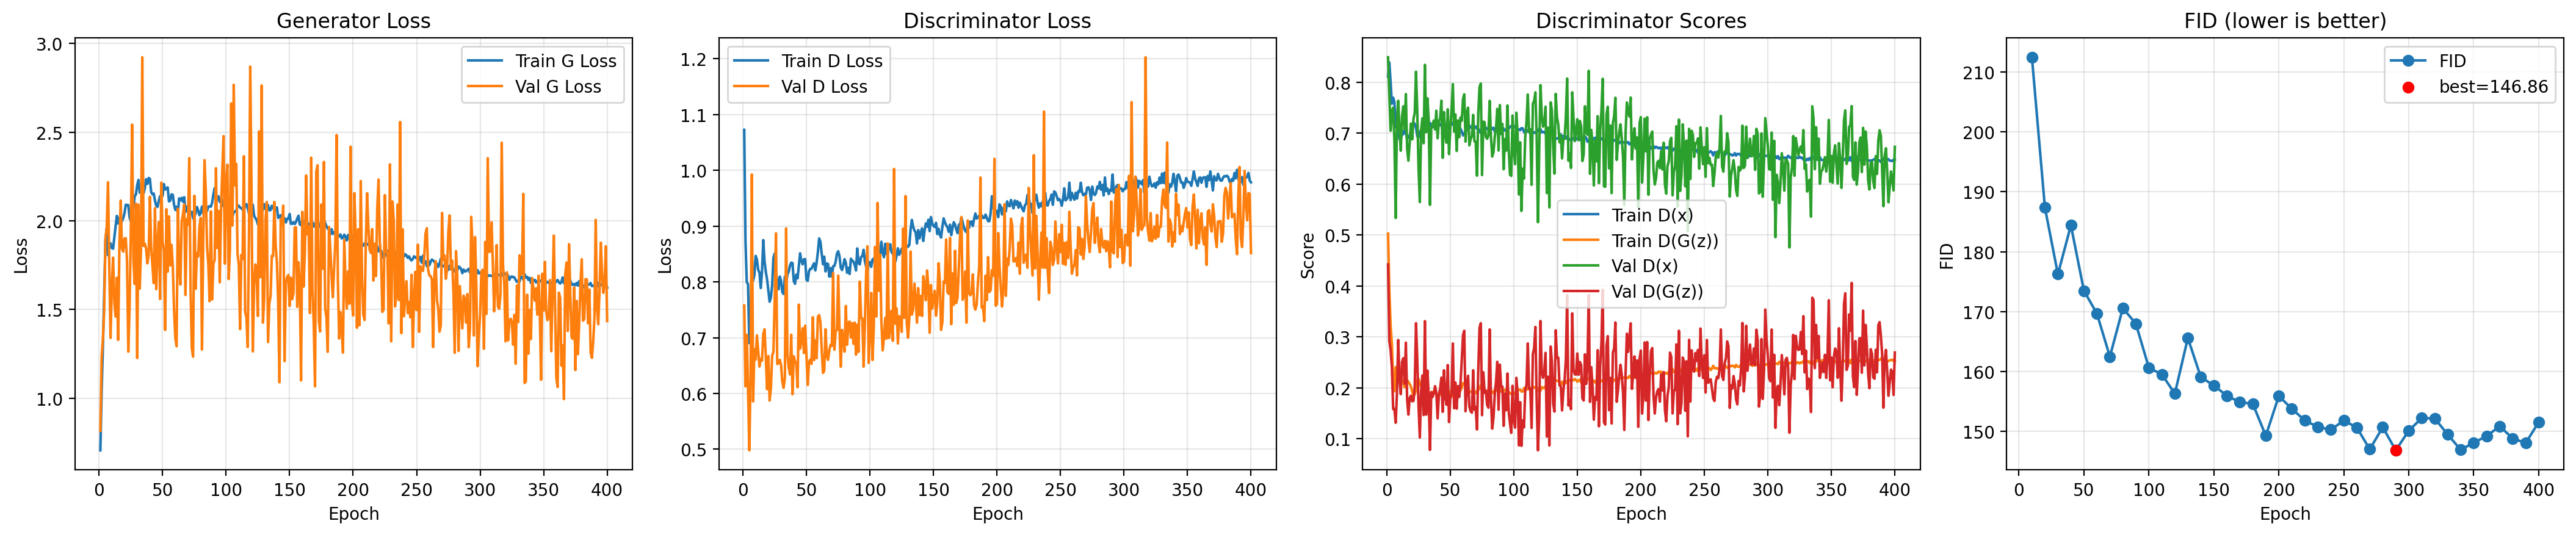
\includegraphics[width=1\textwidth]{gan_training_curves.png}}
    \subfigure[gan\_deep]{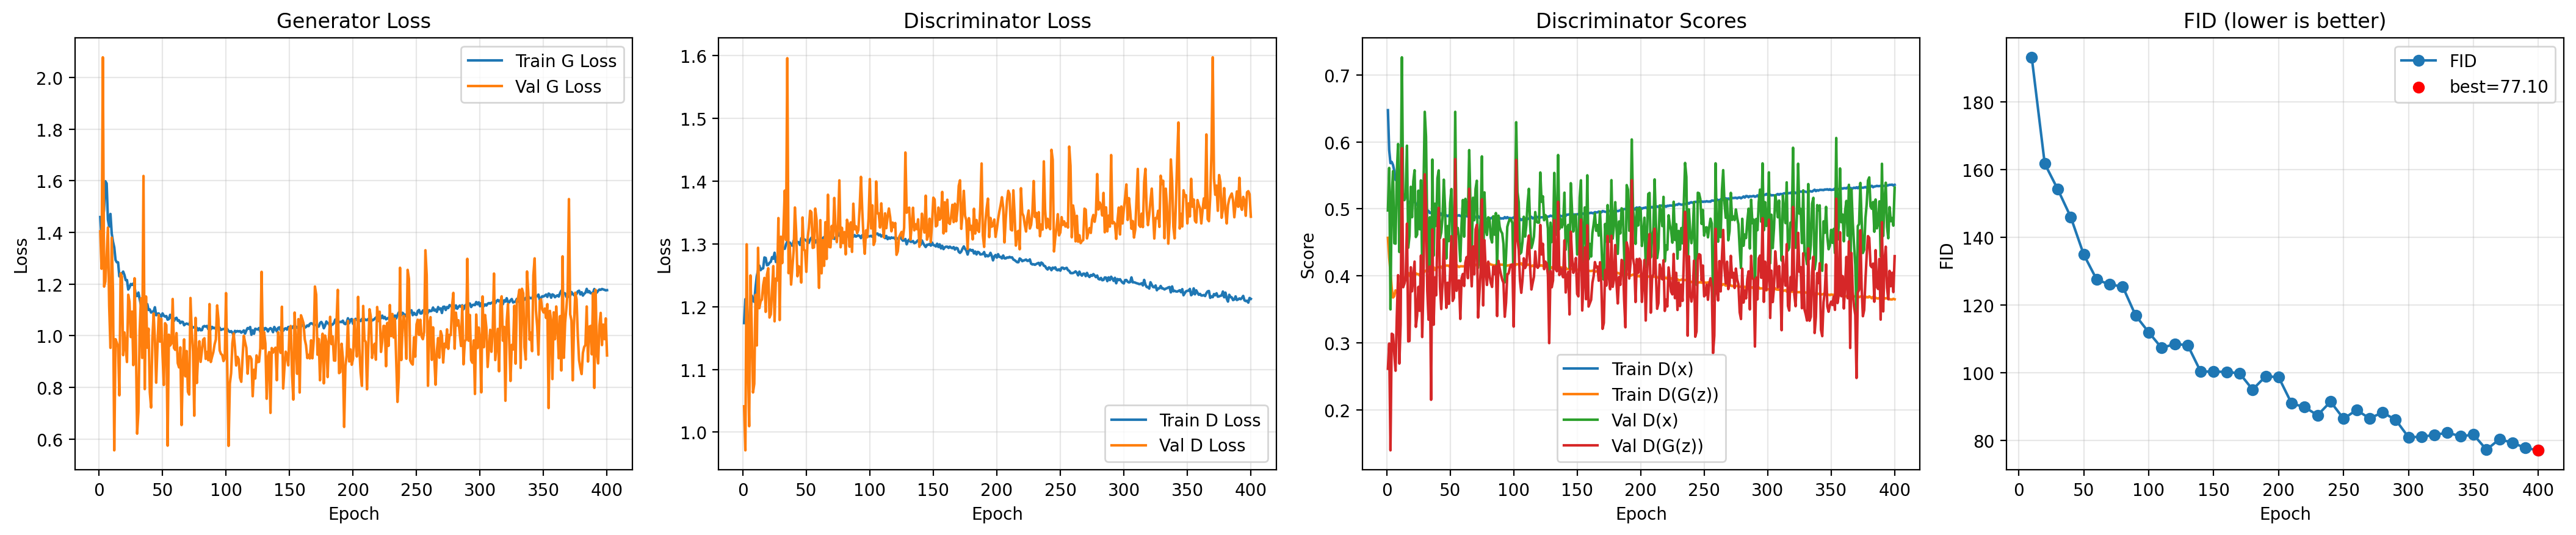
\includegraphics[width=1\textwidth]{gan_deep_training_curves.png}}
    \subfigure[dcgan]{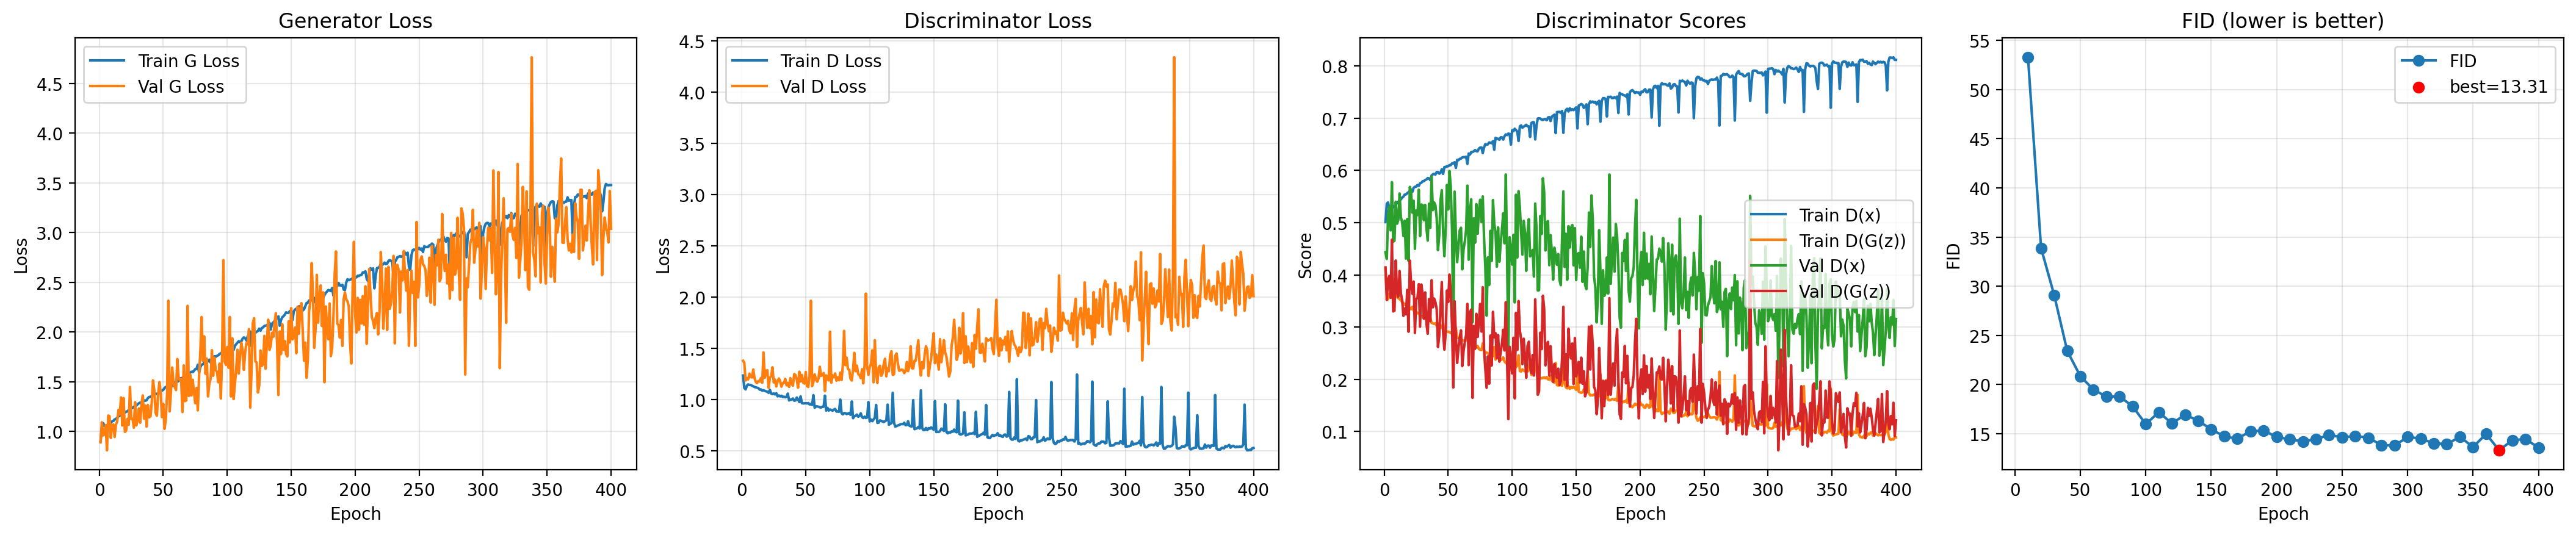
\includegraphics[width=1\textwidth]{dcgan_training_curves.png}}
    \caption{三个模型的训练曲线（G loss / D loss / 判别器打分 / FID）。}
    \label{fig:curves}
\end{figure}

\subsection{训练轮数的影响}
延长训练的收益因模型而异。DCGAN 在 100 轮时 FID 为 21（尚未收敛），延长到 200/400 轮后稳定在 13 附近；优化后的 \texttt{gan\_deep} 在 200 轮到 400 轮间 FID 仍从 93 持续降到 77，且最佳 FID 出现在末轮，说明它在 400 轮内一直未完全收敛、延长仍有收益；而原始 \texttt{gan} 的 FID 在约 290 轮即达到 147 的平台、之后不再下降，说明其瓶颈在网络容量而非训练不足。可见“是否需要延长训练”应结合各模型的收敛曲线判断，而非一概而论。

\subsection{固定噪声生成样例（8 张）}
按要求，固定一组随机噪声，分别输入三个模型的生成器得到样例图（图 \ref{fig:fixed}）。从生成质量看：原始 \texttt{gan} 只能产生模糊轮廓、噪点严重，难以辨认类别；\texttt{gan\_deep} 已能看出上衣、裤子、鞋、包等类别，但表面仍有明显的颗粒状噪声；\texttt{dcgan} 的样例最清晰，衣物边缘锐利、纹理自然，可清楚区分各类衣物。

\begin{figure}[H]
    \centering
    \subfigure[gan]{
\includegraphics[width=0.78\textwidth]{gan_final_gan_fashionmnist_fixed_samples.png}}
    \subfigure[gan\_deep]{
\includegraphics[width=0.78\textwidth]{gan_deep_final_gan_deep_fashionmnist_fixed_samples.png}}
    \subfigure[dcgan]{
\includegraphics[width=0.78\textwidth]{dcgan_final_dcgan_fashionmnist_fixed_samples.png}}
    \caption{三个模型在同一组固定噪声下生成的 8 张样例图对比。}
    \label{fig:fixed}
\end{figure}

\subsection{三种网络生成质量差异分析}
\begin{enumerate}
    \item \textbf{原始全连接 GAN：}生成器仅有单个隐藏层，缺乏对图像空间结构的建模能力，只能学到衣物的粗略灰度分布，因此样例图模糊且噪点多；其最佳 FID 高达 146.9，在三者中最差。这说明在没有空间归纳偏置、容量又很小的情况下，全连接 GAN 难以生成清晰的衣物图像。
    \item \textbf{加深全连接 GAN：}通过加深网络并引入 BatchNorm，\texttt{gan\_deep} 的生成质量明显提升，能够生成可辨认的衣物轮廓，FID 从原始 GAN 的 146.9 降到约 77.1。但由于全连接结构本质上仍把图像当作一维向量处理、缺乏局部相关性建模，其生成图始终带有椒盐状噪声，质量存在上限。
    \item \textbf{卷积 DCGAN：}卷积/转置卷积显式建模了局部空间相关性，因此 DCGAN 的 FID 明显领先（约 13.3，比 \texttt{gan\_deep} 低近一个数量级），生成图最清晰。这说明卷积结构对图像生成任务具有关键作用。
\end{enumerate}

值得强调的一个现象是：\texttt{gan\_deep} 在训练过程中 $D(x)$、$D(G(z))$ 最接近理论均衡（约 0.5），即从“对抗均衡”角度看它最“健康”，但其生成质量（FID）却明显不如判别器一度占优的 DCGAN。这再次说明对抗 loss 的均衡程度并不等价于生成质量，必须借助 FID 这类样本级指标来评估。

\section{隐变量扰动对生成结果的影响}
\label{sec:latent}
\subsection{分析方法}
固定一组 100 维随机噪声向量（共 8 个样本），从中挑选 5 个对生成结果影响最大的“活跃”维度——由于隐空间各向异性，多数维度对输出几乎无影响，若随机挑选很容易选到这类“不活跃维度”而看不出变化，因此先逐维施加扰动、按生成图的平均变化幅度排序，取影响最大的 5 个维度。对每个被选维度施加 3 档扰动（$-2.5$、$0$、$+2.5$），其余维度保持不变，从而观察“仅改变单个随机数”时生成图像的变化。每个维度的 3 档扰动 $\times$ 8 个样本构成一行组，5 个维度共得到 $15\times8$ 张图像，如图 \ref{fig:latent} 所示。

\begin{figure}[H]
    \centering
    \subfigure[gan]{
\includegraphics[width=0.32\textwidth]{gan_final_gan_fashionmnist_latent_variations.png}}
    \subfigure[gan\_deep]{
\includegraphics[width=0.32\textwidth]{gan_deep_final_gan_deep_fashionmnist_latent_variations.png}}
    \subfigure[dcgan]{
\includegraphics[width=0.32\textwidth]{dcgan_final_dcgan_fashionmnist_latent_variations.png}}
    \caption{三个模型的隐变量扰动分析（每图 $15\times8$：5 个维度 $\times$ 每维 3 档扰动 $\times$ 8 个固定样本）。}
    \label{fig:latent}
\end{figure}

\subsection{扰动现象与解释}
从图 \ref{fig:latent} 可以观察到以下现象：
\begin{enumerate}
    \item \textbf{单维扰动的影响：}在选取了活跃维度并加大扰动幅度后，单个维度的变化已能引起明显的视觉变化——衣物的明暗深浅、厚度、轮廓胖瘦乃至在相近类别之间（如上衣与外套、鞋型之间）的过渡都会随之改变。这说明这些维度确实“活跃”，但单个维度往往同时牵动多个属性，并不对应某一个清晰可解释的语义。
    \item \textbf{潜空间的纠缠性：}与 StyleGAN\cite{karras2019stylegan} 等具有解耦隐空间的模型不同，原始 GAN/DCGAN 的隐空间是高度纠缠的——单个维度的语义并不独立，改变一个维度往往同时引起多个视觉属性的整体性变化，且不同样本上同一维度的作用方向也不一致。因此普通 GAN 上很难找到“某一维就是亮度、某一维就是袖长”这种清晰对应，这也是普通 GAN 隐变量难以独立解释、扰动效果偏整体的根本原因。
    \item \textbf{模型差异：}对比三个模型可见，\texttt{dcgan} 的扰动变化最平滑、可读性最好；\texttt{gan\_deep} 能反映扰动但带有明显的颗粒噪声；而优化后的原始 \texttt{gan} 因模式崩溃，各样本本身就高度相似（多为上衣类），即便扰动活跃维度，变化也最有限。
\end{enumerate}

综合来看，隐变量扰动实验说明：在不加解耦约束的普通 GAN 中，隐空间各维度与可见语义属性之间不是一一对应关系，而是以纠缠方式共同决定生成结果；要获得可解释、可独立操控的隐变量，需要引入额外的解耦机制（如条件输入或风格解耦结构），这可作为后续改进方向。

\section{进阶分析}
为更深入地理解三个模型，参考 DCGAN 论文\cite{radford2015dcgan}补充了四组分析实验，均基于训练好的最终模型。

\subsection{潜空间插值}
借助分类器筛选出分别生成“鞋”和“衣物”且置信度较高的两个端点噪声 $z_1,z_2$，在两者之间线性插值 10 步，每个模型展示一行（图 \ref{fig:interp}）。若过渡平滑连续，说明生成器学到的是连续的数据流形，而非记忆训练样本。可以看到：\texttt{dcgan} 从凉鞋平滑过渡到长袖上衣，中间形态自然连续，过渡质量最好；\texttt{gan\_deep} 也能完成凉鞋到连衣裙的过渡，但中间态带有噪点；而原始 \texttt{gan} 由于模式崩溃，连“鞋”端点都只能勉强生成（分类器置信度仅 0.65），整行都是模糊的上衣/连衣裙、缺乏清晰的跨类别过渡，印证其隐空间已严重退化（这与第 \ref{sec:diversity} 节的多样性结论一致）。这说明卷积/加深结构学到了更光滑、更有结构的隐空间映射。

\begin{figure}[H]
    \centering
    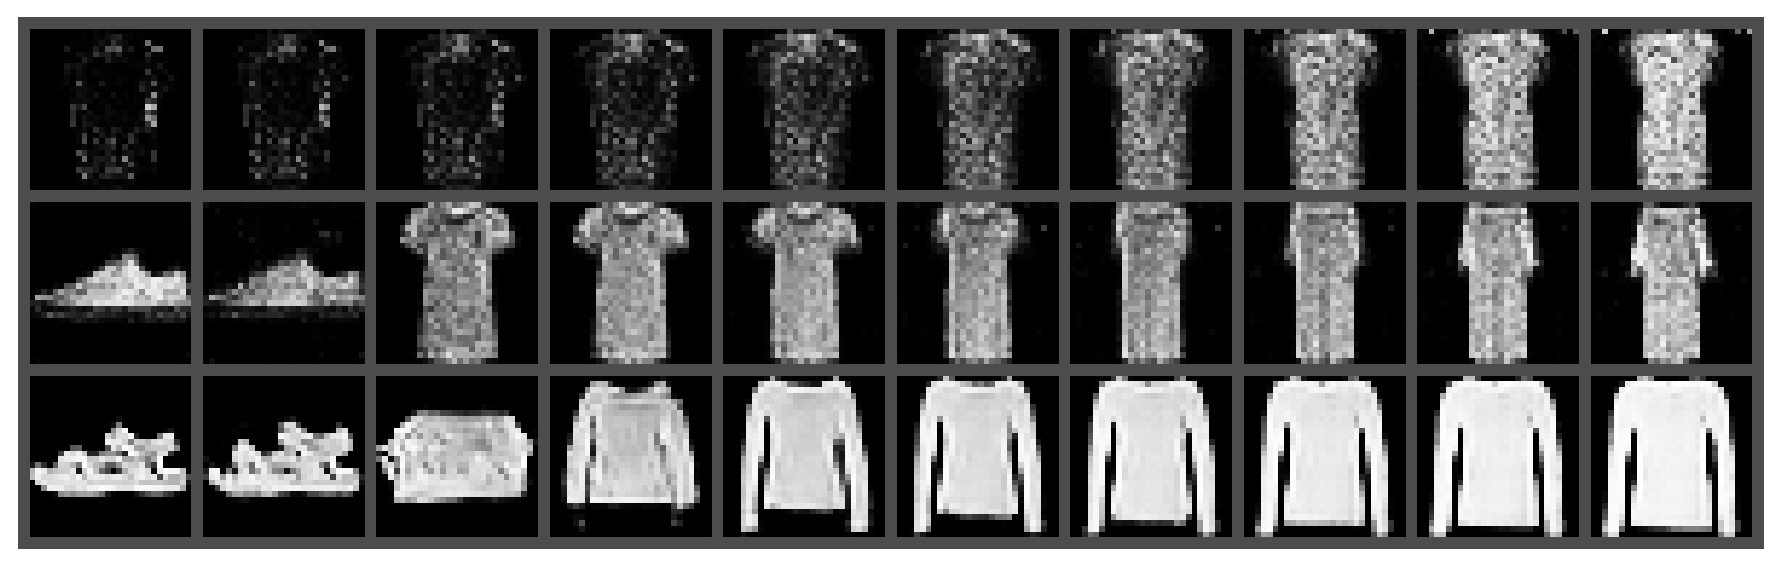
\includegraphics[width=0.92\textwidth]{interpolation_grid.png}
    \caption{潜空间插值：每行一个模型（自上而下为 gan、gan\_deep、dcgan），从左到右为“鞋 $\rightarrow$ 衣物”的 10 步线性插值。}
    \label{fig:interp}
\end{figure}


\subsection{生成多样性与模式崩溃}
\label{sec:diversity}
模式崩溃是 GAN 的典型失败模式，而 FID 主要衡量分布距离、对“多样性”不够敏感。为此训练了一个 FashionMNIST 分类器（测试准确率约 89\%，实现见附录 \ref{app:clf}）作为裁判，对每个生成器采样 5000 张图分类，统计生成样本在 10 个类别上的分布（图 \ref{fig:diversity}）。结果显示：原始 \texttt{gan}（优化后）的归一化熵仅 0.693、只覆盖 6/10 个类别，出现了明显的模式崩溃（严重偏向生成 Shirt，占 38\%）——这正是附录 \ref{sec:opt} 提到的权衡：TTUR 强化判别器后，容量极弱的生成器只能靠生成少数“安全”类别来压低 FID；相比之下 \texttt{gan\_deep} 与 \texttt{dcgan} 都覆盖全部 10 类，其中 \texttt{dcgan} 的归一化熵高达 0.999，分布几乎完全均匀，多样性最好。这从“多样性”角度补充了 FID 的结论，也说明 FID 低并不等于多样性好。

\begin{figure}[H]
\centering
\begin{minipage}[c]{0.52\textwidth}
    \centering
    
\includegraphics[width=\textwidth]{diversity_class_distribution.png}
\end{minipage}\hfill
\begin{minipage}[c]{0.45\textwidth}
    \centering
    \small
    \begin{tabular}{lccc}
    \toprule
    Model & 熵 $\uparrow$ & 覆盖类 & 最多类 \\
    \midrule
    gan      & 0.693 & 6/10 & Shirt(.38) \\
    gan\_deep & 0.965 & 10/10 & Shirt(.19) \\
    dcgan    & \textbf{0.999} & 10/10 & Sandal(.11) \\
    \bottomrule
    \end{tabular}
\end{minipage}
\caption{三个模型生成样本在 10 个类别上的分布：雷达图（左）与统计表（右）。\texttt{gan} 明显集中于 Shirt（模式崩溃），\texttt{dcgan} 分布最均匀。}
\label{fig:diversity}
\end{figure}


\subsection{最近邻过拟合检验}
为验证生成器是否只是“记住”了训练样本，将生成图在训练集中检索 L2 距离最近的真实图并排展示（图 \ref{fig:nn}，上行为生成图、下行为对应的最近邻真实图）。可以看到，生成图与其最近邻真实图属于同一类别但细节明显不同（并非同一张图的复制），说明模型确实在生成新样本，而非过拟合/记忆训练集。

\begin{figure}[H]
    \centering
    
\includegraphics[width=0.72\textwidth]{dcgan_nearest_neighbor.png}
    \caption{DCGAN 生成图（上行）与训练集中 L2 最近邻真实图（下行）对照。}
    \label{fig:nn}
\end{figure}


\subsection{判别器特征的表示学习能力}
DCGAN 论文的一个重要论点是：对抗训练能让判别器无监督地学到有用的特征表示\cite{radford2015dcgan}。为此冻结训练好的判别器，取其最后分类层之前的特征，训练一个线性分类器在 FashionMNIST 上分类，并与“原始像素”和“随机初始化判别器”两个基线对比（表 \ref{tab:probe}）。结果显示，DCGAN 的卷积判别器训练后特征（87.9\%）显著超过原始像素（83.5\%）和随机初始化判别器（69.6\%），证明对抗训练让卷积判别器学到了比原始像素更有判别力的语义特征；优化后的 \texttt{gan\_deep} 判别器（去掉 Dropout、判别器更强）特征也达到 86.1\%、略超原始像素；而原始 \texttt{gan} 判别器（82.3\%）仍不及像素。可见判别器能否学到优于像素的表示，与其容量和训练是否充分密切相关，其中 DCGAN 的卷积结构优势最明显。这与生成端 DCGAN 远优于全连接 GAN 的结论相互印证。

\begin{table}[H]
\centering
\caption{判别器特征的线性探针准确率（冻结特征 + 线性分类器，FashionMNIST 测试集）。原始像素为不经过判别器的参照基线，无“训练后/随机初始化”之分，故只有一个值。}
\begin{tabular}{lcc}
\toprule
特征来源 & 训练后判别器 & 随机初始化判别器 \\
\midrule
原始像素 baseline & \multicolumn{2}{c}{0.835} \\
gan 判别器 (128 维) & 0.823 & 0.777 \\
gan\_deep 判别器 (256 维) & 0.861 & 0.756 \\
dcgan 判别器 (256 维) & \textbf{0.879} & 0.696 \\
\bottomrule
\end{tabular}
\label{tab:probe}
\end{table}

\section{实验结论}
本文在 FashionMNIST 上实现并对比了原始全连接 GAN、加深全连接 GAN 与卷积版 DCGAN，并以 FID 作为统一的质量评价指标。实验结果表明：（1）三个模型呈现明显的质量递进，DCGAN 的 FID 显著优于两种全连接 GAN，体现了卷积结构对图像生成的关键作用；（2）对抗 loss 的均衡程度并不等价于生成质量，FID 等样本级指标对 GAN 评估是必要的；（3）训练轮数的影响因模型而异，DCGAN 从延长训练中获益明显，而容量受限的原始 GAN 延长训练并无帮助；（4）普通 GAN 的隐空间高度纠缠，单个随机数的扰动以整体方式影响生成结果，难以对应到独立的语义属性。针对全连接 GAN 判别器过早饱和的问题，本文通过去除判别器 Dropout、TTUR 与单边标签平滑进行优化，并将训练延长到 400 轮，使 \texttt{gan\_deep} 的 FID 从 115.7 降到 77.1，但也观察到对容量极弱的原始 GAN，强化判别器会带来 FID 与多样性之间的权衡。此外，进阶实验进一步表明：潜空间插值在 DCGAN 上呈现平滑过渡，说明其学到了连续流形；多样性统计显示原始 GAN 出现明显的模式崩溃（仅覆盖 6/10 类）而 DCGAN 分布几乎完全均匀；最近邻检验排除了记忆训练集的可能；判别器特征的线性探针则表明卷积判别器学到的特征最有判别力、明显优于原始像素（加深的全连接判别器也略超像素）。总体而言，本实验完整覆盖了作业要求的 loss 曲线、模型结构、固定噪声样例与隐变量扰动分析，并通过 FID、多样性、表示学习等多个维度对 GAN 的训练与评估进行了较深入的探讨。

\newpage

\appendix
\section{训练诊断与优化}
\label{sec:opt}
正文中两个全连接 GAN 的最终模型均采用了本节所述的优化配置，其动机来自对标准训练过程的观察。

在标准训练下，\texttt{gan\_deep} 的判别器损失很快升到约 $2\log 2\approx1.386$，且 $D(x)\approx D(G(z))\approx 0.5$，即判别器已被“打平”、无法区分真假。由于生成器的梯度完全来自判别器，判别器一旦失效，生成器便失去了有效的训练信号，这正是其 FID 在约 115 处过早进入平台的原因。究其根源，是判别器相对生成器太弱：不仅参数更少，隐藏层中的两个 $\text{Dropout}(0.3)$ 还进一步削弱了它。

据此，对两个全连接 GAN 施加了三项调整：去掉判别器的 Dropout；采用 TTUR\cite{heusel2017fid}，让判别器使用更高的学习率（$5\times10^{-4}$）、生成器使用较低的学习率（$2\times10^{-4}$）；以及单边标签平滑，将真实标签取为 0.9。优化后 \texttt{gan\_deep} 的判别器损失不再饱和（维持在约 1.3），$D(G(z))<D(x)$，重新具备了区分能力，FID 也持续下降、到 400 轮仍未见明显平台。

优化前后的最佳 FID 对比见表 \ref{tab:opt}：\texttt{gan\_deep} 改善了近 20\%，\texttt{gan} 也有小幅改善，验证了“判别器过早饱和”这一诊断。在此基础上将训练延长到 400 轮，\texttt{gan\_deep} 的 FID 进一步降到 77.1、\texttt{gan} 降到 146.9，正文最终模型即采用 400 轮的结果。不过需要指出一个权衡：原始 \texttt{gan} 优化后虽然 FID 略有下降，其生成多样性却反而变差（见第 \ref{sec:diversity} 节）——TTUR 把判别器催得过强，迫使本就很弱的生成器进一步崩溃到少数类别。可见同一套优化手段对不同容量的模型效果并不相同，调优需结合模型自身的能力来权衡。

\begin{table}[H]
\centering
\caption{训练优化前后的最佳 FID 对比（越低越好）}
\begin{tabular}{lccc}
\toprule
Model & 标准训练 FID & 优化后 FID & 相对改善 \\
\midrule
gan      & 161.8 & 154.3 & $-5\%$ \\
gan\_deep & 115.7 & \textbf{93.3} & $\mathbf{-19\%}$ \\
\bottomrule
\end{tabular}
\label{tab:opt}
\end{table}

\section{评估指标的探索过程}
\label{app:metric}
在确定采用 FID 之前，本文曾尝试用一个“对抗均衡分”来选择 checkpoint，即衡量生成器损失、判别器损失与 $D(x)$、$D(G(z))$ 偏离理论均衡点（分别为 $\log 2$、$2\log 2$、$0.5$、$0.5$）的程度，分数越低代表越接近理想的对抗博弈状态。

但实践中发现该指标存在系统性缺陷：训练初期生成器与判别器都接近随机状态（判别器对真假样本都输出约 0.5、损失也接近理论均衡值），均衡分反而最低，因此它会把几乎没有训练的早期 epoch 误判为最优。一个典型例子是 DCGAN：按均衡分会选到学习率 $0.0001$、且最佳轮次仅为第 2 轮的 checkpoint，而该学习率的实际 FID 在四个候选中最差；相比之下，FID 正确地选出了收敛更充分的 $0.0005$。由于这一缺陷，最终放弃了该启发式，改以 FID 作为唯一的模型选择与超参选择依据。

\section{多样性评估所用的 FashionMNIST 分类器}
\label{app:clf}
第 \ref{sec:diversity} 节的多样性评估，以及附录中潜空间插值的端点筛选，都用到了一个分类器作为“裁判”。该分类器是一个简单 CNN：两层卷积（卷积核 $3\times3$，输出通道分别为 32、64，每层后接 ReLU 与 $2\times2$ 最大池化）后接两层全连接（$128$ 维隐层 + $10$ 类输出），在 FashionMNIST 训练集上用 Adam（学习率 $10^{-3}$）训练 3 个 epoch，测试集准确率约 89\%。在多样性实验中，用它对每个生成器的 5000 张生成图进行分类，统计 10 个类别上的分布；在插值实验中，用它筛选出分别生成“鞋”和“衣物”的端点噪声。

\section{网络结构的完整 \texttt{print(net)} 输出}
\label{app:prints}
下面给出三个模型生成器与判别器完整的 \texttt{print(net)} 输出，对应正文表 \ref{tab:model_prints} 的结构骨架。

\lstinputlisting[basicstyle=\scriptsize\ttfamily,frame=single,breaklines=true]{model_prints/gan_print.txt}
\lstinputlisting[basicstyle=\scriptsize\ttfamily,frame=single,breaklines=true]{model_prints/gan_deep_print.txt}
\lstinputlisting[basicstyle=\scriptsize\ttfamily,frame=single,breaklines=true]{model_prints/dcgan_print.txt}

\section{代码目录说明}
本实验代码位于 \texttt{lab4/} 目录，核心文件如下：
\begin{itemize}
    \item \texttt{train.py}：单次训练入口；
    \item \texttt{sweep\_lr.py}：学习率扫描入口（按 FID 选最优学习率）；
    \item \texttt{src/models/}：模型实现，含 \texttt{gan.py}（原始与加深全连接 GAN）、\texttt{dcgan.py}（卷积版）、\texttt{registry.py}（统一构建与权重初始化）；
    \item \texttt{src/engine.py}：训练/验证/测试主循环，含按 FID 选 checkpoint 的逻辑；
    \item \texttt{src/utils/fid.py}：基于 Inception-V3 的 FID 评估器；
    \item \texttt{src/data.py}：FashionMNIST 数据加载与划分；
    \item \texttt{scripts/generate\_report\_assets.py}：报告图表（固定噪声样例、隐变量扰动图、指标表）生成；
    \item \texttt{scripts/advanced\_analysis.py}：进阶分析（潜空间插值、多样性/模式崩溃、最近邻检验、判别器特征线性探针）；
    \item \texttt{scripts/run\_lab4\_2gpu.sh}、\texttt{scripts/run\_lab4\_final400.sh}：双卡总控与 400 轮最终训练脚本。
\end{itemize}

\bibliographystyle{plain}
\bibliography{reference}

\end{document}
